\documentclass[a4paper]{article}

%%%%%%%%%%%%%%%%%%%%%%%%%%%%%%%%%%%%%%%%%%%%%%
\usepackage[T1]{fontenc}
\usepackage{geometry}
\geometry{a4paper,left=1.5cm,right=1cm,top=1cm,bottom=1cm}

\usepackage{graphicx}
\usepackage[absolute,overlay]{textpos}
\usepackage{eso-pic}               % image de fond
\usepackage{fontawesome5}
\usepackage[hidelinks]{hyperref}
\usepackage{tikz}
\usepackage{xcolor}
\usepackage{enumitem}
\setlist{nosep,leftmargin=6mm}
\usepackage{times}                % même police que votre exemple
\usepackage{array} 
\usepackage{tabularx}
\usepackage{ragged2e}

%%%%%%%%%%%%%%%%%%%%%%%%%%%%%%%%%%%%%%%%%%%%%%
%\definecolor{texcolor}{HTML}{e2e8f0}
\providecolor{sidetext}{rgb}{0,0,0}
\definecolor{maincolor}{HTML}{ffffff}

%%%%%%%%%%%%%%%%%%%%%%%%%%%%%%%%%%%%%%%%%
% — Ne changez pas le nom : « background.jpg » doit être présent
\AddToShipoutPictureBG*{%
  
\includegraphics[width=\paperwidth,height=\paperheight]{background.jpg}%
}

%%%%%%%%%%%%%%%%%%%%%%%%%%%%%%%%%%%%%%%%%
\newcommand{\fullrule}{\hspace{-1.5cm}\rule{\paperwidth}{0.4pt}}
\newcommand{\cvsection}[1]{%
  \vspace{6pt}\textbf{\Large #1}\par\vspace{2pt}}
\newcommand{\cicon}[1]{%
  \tikz[baseline]{\draw[fill=white] (0,0.1) circle[radius=0.1cm];}~#1}

\setlength{\parindent}{0pt}
%\color{texcolor}
%%%%%%%%%%%%%%%%%%%%%%%%%%%%%%%%%%%%%%%%%%%%%%%%%%%%%%%%%%%%%%
\begin{document}

% ---------- Photo ------------------------------------------------
\begin{textblock*}{4cm}(0.2cm,0.3cm)
  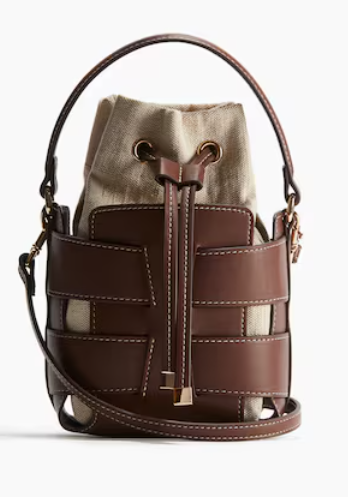
\includegraphics[width=2.5cm,clip,keepaspectratio]{595b9176264f479bb08deb31070e3c8d.png}
\end{textblock*}

% ---------- En-tête ---------------------------------------------
\begin{center}
  {\fontsize{44pt}{24pt}\selectfont\bfseries Judikael Mourouvin}

  \bigskip
  {\Large Technicien informatique \& marketing digital}

  \bigskip\bigskip
  \faMapMarker~Route de COCOYER\ 97190 GOSIER
  \quad\faEnvelope~\href{mailto:jkmou971@gmail.com}{jkmou971@gmail.com}

  \bigskip
  % Badge LinkedIn (retirez-le si inutile)
  
\begin{tikzpicture}
    \node[draw,fill=white,rounded corners=9pt,inner xsep=8pt,inner ysep=4pt]
         {\color{black}\faLinkedin\ \href{}{}};
  \end{tikzpicture}

  \vspace{-0.3cm}
  \fullrule
\end{center}

% ---------- Profil ----------------------------------------------
\cvsection{Profil}
Passionné par l’informatique et le marketing digital, je maîtrise la configuration de postes, la maintenance matérielle et la résolution d’incidents. Mon alternance à la DSI de la Mairie du Gosier m’a permis de gérer des projets numériques et d’accompagner les utilisateurs au quotidien. J’ai également développé une solide expérience en support technique et en animation d’espaces informatiques chez Pôle Emploi. Désormais, je souhaite mettre mon sens du service et ma rigueur au service d’une équipe à temps plein.

\medskip\fullrule

% ---------- Éducation -------------------------------------------
\cvsection{Éducation}

    \begin{tabularx}{\linewidth}{@{}c >{\RaggedRight\arraybackslash}X@{}}
    \textcolor{sidetext}{\faGraduationCap} &
    \textbf{Bachelor Marketing Digital} \\
    & CFA IUTS \\
    & \textit{2023-2024} \\
    \end{tabularx}
    \begin{itemize}[leftmargin=*]
  \item Acquisition des fondamentaux du marketing numérique : SEO, SEA, réseaux sociaux.
  \item Gestion de projet digital et analyse de données marketing.
  \item Élaboration de stratégies de communication en ligne.
\end{itemize}
\vspace{3mm}

    \begin{tabularx}{\linewidth}{@{}c >{\RaggedRight\arraybackslash}X@{}}
    \textcolor{sidetext}{\faGraduationCap} &
    \textbf{BTS Systèmes Numériques option Informatique et Réseaux} \\
    & Lycée de Chevalier Saint Georges, Abymes \\
    & \textit{2019-2021} \\
    \end{tabularx}
    \begin{itemize}[leftmargin=*]
  \item Étude des architectures réseaux et systèmes informatiques.
  \item Pratique de la maintenance matérielle et logicielle.
  \item Mise en œuvre de projets liés à la cybersécurité et au support utilisateur.
\end{itemize}

\medskip\fullrule

% ---------- Expérience ------------------------------------------
\cvsection{Expérience}

\colorbox{maincolor}{%
  \begin{minipage}{\linewidth}
    \textbf{Alternant en marketing digital} \\ Mairie du Gosier – DSI \\ 2023-2024
    \begin{itemize}
      \item Géré des projets numériques municipaux, assurant leur déploiement dans les délais. \item Analysé les besoins des agents et implémenté des solutions adaptées, améliorant l’efficacité des services. \item Assuré support et formation, renforçant l’adoption des outils digitaux.
    \end{itemize}
  \end{minipage}}

\vspace{3mm}


\colorbox{maincolor}{%
  \begin{minipage}{\linewidth}
    \textbf{Animateur de la zone informatique} \\ Pôle Emploi, Gosier \\ 2022-2023
    \begin{itemize}
      \item Offert un support de proximité à des demandeurs d’emploi, réduisant les temps d’attente. \item Configuré et entretenu le parc informatique, garantissant la disponibilité des postes. \item Diagnostiqué et résolu les incidents, assurant la continuité du service.
    \end{itemize}
  \end{minipage}}

\vspace{3mm}


\colorbox{maincolor}{%
  \begin{minipage}{\linewidth}
    \textbf{Stagiaire informaticien} \\ NUMERIKA, Baie Mahault \\ 2020-2021
    \begin{itemize}
      \item Installé et configuré des équipements, optimisant les performances du réseau interne. \item Réalisé la maintenance préventive du matériel, limitant les pannes. \item Fournit un support quotidien aux utilisateurs, améliorant leur productivité.
    \end{itemize}
  \end{minipage}}

\medskip\fullrule

% ---------- Compétences -----------------------------------------
\cvsection{Compétences}
\begin{tabular}{@{}p{0.25\linewidth}p{0.18\linewidth}p{0.18\linewidth}p{0.18\linewidth}}\cicon Administration & \cicon Maintenance & \cicon Réseaux & \cicon Assistance \\
\cicon Support & \cicon Diagnostic & \cicon Configuration & \cicon Marketing \\
\cicon Digital & \cicon Analyse & ~ & ~ \\\end{tabular}   % grille 3 lignes × 4 colonnes

\end{document}
